\documentclass[11pt,oneside]{memoir}
\usepackage{iftex}
\ifPDFTeX
  \usepackage[T1]{fontenc}
  \usepackage{lmodern}
\else
  \usepackage{fontspec}
  \setmainfont{Latin Modern Roman}
  \setsansfont{Latin Modern Sans}
  \setmonofont{Latin Modern Mono}
\fi
\usepackage[english]{babel}
\usepackage{xcolor}
\usepackage{graphicx}
\usepackage[section]{placeins}
\usepackage{array}
\usepackage{booktabs}
\usepackage{longtable}
\usepackage{tabularx}
\usepackage{enumitem}
\usepackage{fvextra}
\usepackage{microtype}
\usepackage{hyperref}
\usepackage{bookmark}
\usepackage{listings}
\graphicspath{{figures/}}
\definecolor{manualblue}{HTML}{174A7E}
\hypersetup{colorlinks=true,linkcolor=manualblue,urlcolor=manualblue,citecolor=manualblue}
\setstocksize{11in}{8.5in}
\settrimmedsize{\stockheight}{\stockwidth}{*}
\setlrmarginsandblock{1in}{1in}{*}
\setulmarginsandblock{1in}{1in}{*}
\setlength{\headheight}{30pt}
\checkandfixthelayout
\chapterstyle{section}
\setsecnumdepth{subsection}
\setsecheadstyle{\Large\bfseries\color{manualblue}}
\setsubsecheadstyle{\large\bfseries\color{manualblue}}
% Define a custom color for the terminal background
\definecolor{termbg}{rgb}{0.95, 0.95, 0.95}
\lstset{
    backgroundcolor=\color{gray!5},
    basicstyle=\small\ttfamily,
    breaklines=true,
    keywordstyle=\color{blue},
    commentstyle=\color{gray},
    stringstyle=\color{purple},
    frame=single
}
% Configure the terminal style
\lstdefinestyle{terminal}{
    backgroundcolor=\color{termbg},   % Light grey background
    basicstyle=\small\ttfamily,       % Monospace font for commands
    breaklines=true,                  % Automatically wrap long lines
    frame=single,                     % Draw a box around the code
    frameround=tttt,                  % Slightly rounded corners for the frame
    framesep=5pt,                     % Padding inside the frame
    rulecolor=\color{gray!40},        % Border color
    upquote=true                      % Prevents straight quotes from curling
}

\setlength{\parindent}{0pt}
\setlength{\parskip}{0.55em}
\setlist[itemize]{leftmargin=2em,itemsep=0.15em,topsep=0.25em}
\newcommand{\manualtitle}{CU-AIM Server User Manual 2026}
\title{\manualtitle}
\author{}
\date{}
\begin{document}
\hypersetup{pageanchor=false}
\frontmatter
\begin{titlingpage}
\centering
\vspace*{0.22\textheight}
{\Huge\bfseries\color{manualblue}\manualtitle\par}
\vspace{1.5em}
{\Large A practical CU-AIM server guide for our lab users\par}
{Link for related codes: \url{github_placeholder}\par}
{Last Updated: 11/09/2026\par}
\vfill

\par
Created by Peeradon Sarnkaew 
\par
Contact Email: peeradonsarnkaew46@gmail.com
\par

\end{titlingpage}
\hypersetup{pageanchor=true}
\tableofcontents*
\mainmatter




\chapter{Prepare First-Time Access}
\label{chap:first-time-setup}
This manual introduces the routine workflow for using the CU-AIM computing cluster. A cluster is a shared group of computers managed by a scheduler, which assigns resources to submitted work. The manual is intended for students who are familiar with basic files and Python but are new to remote servers and Slurm.

Complete this chapter once on each computer that you will use to access CU-AIM. The normal order is to connect to the university VPN, create an SSH key pair, submit the public key for authorization, and then test the connection.

\section{Connect to the Chula VPN}
\label{sec:connect-vpn}
\begin{enumerate}
\item Download and install Cisco AnyConnect by following the Chulalongkorn University IT instructions: \url{https://www.it.chula.ac.th/en/service/en-vpn/}.

\item Open Cisco AnyConnect and enter the VPN server given in the current university instructions. Sign in with your Chula username and password. \textbf{You have to connect to this VPN every time you want to use the CUAIM server!}
\begin{figure}[!htbp]
\centering

\includegraphics[width=0.7\linewidth,keepaspectratio]{figures/cisco_vpn.png}
\caption{Cisco AnyConnect VPN connection settings.}
\label{fig:cisco-vpn}
\end{figure}
\end{enumerate}

\section{Create an SSH Key Pair}
\label{sec:ssh-keys}
CU-AIM uses SSH public-key authentication. An SSH key pair contains a public key that you may share and a private key that must remain on your computer. Never send your private key to another person or store it in a shared project directory.

Choose either the PuTTY method or the terminal method below. You do not need to use both.

\subsection{Generate a Key with PuTTY}
\label{subsec:generate-ssh-keys}
\label{subsubsec:generate-putty}

The walkthrough video at \url{https://youtu.be/atx3VhDUOr8} demonstrates this process. The essential steps are summarized here.
\begin{enumerate}
  \item Download and install PuTTY from \url{https://www.putty.org/}.
  \item Open PuTTYgen, select the settings shown in Figure~\ref{fig:puttygen-settings}, and click \textbf{Generate}.
  \begin{figure}[!htbp]
\centering
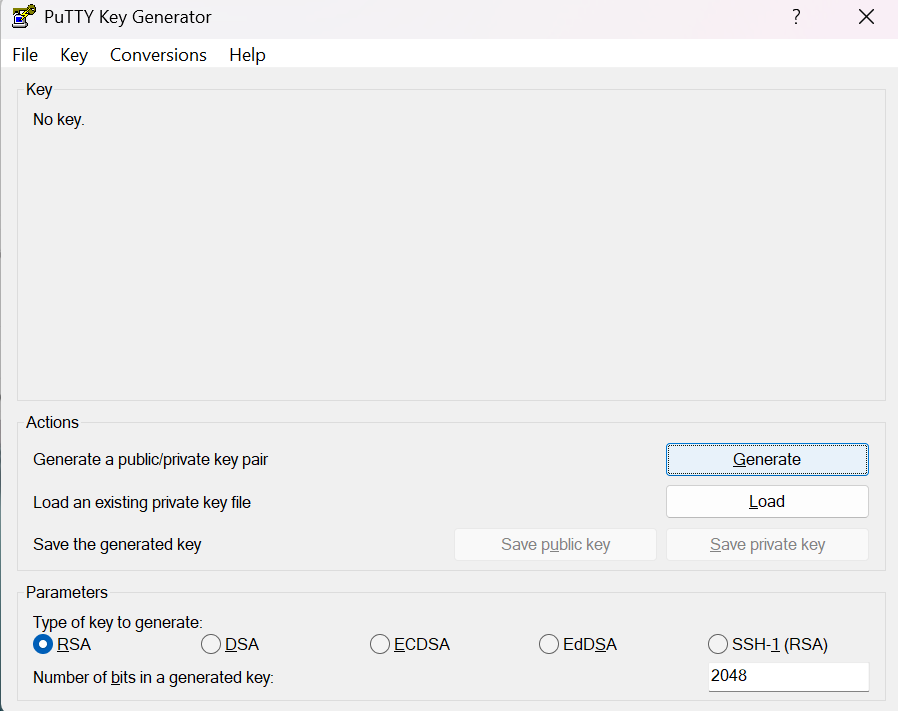
\includegraphics[width=0.8\linewidth,keepaspectratio]{figures/image-01.png}
\caption{PuTTYgen key-generation settings.}
\label{fig:puttygen-settings}
\end{figure}

  \item Move the pointer over the blank area until PuTTYgen finishes creating the key.
  \begin{figure}[!htbp]
\centering
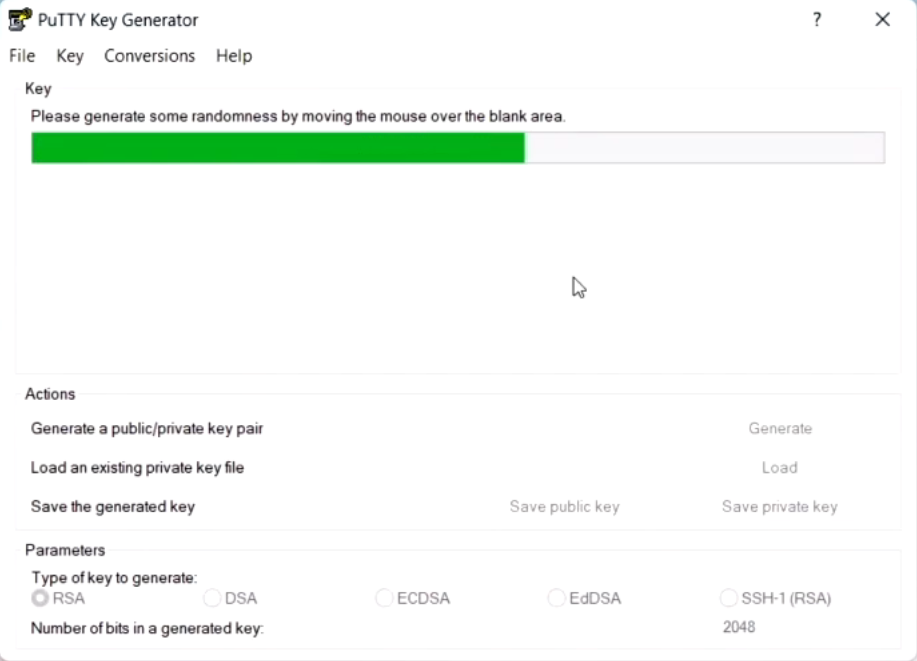
\includegraphics[width=0.8\linewidth,keepaspectratio]{figures/image-02.png}
\caption{PuTTYgen generating an SSH key.}
\label{fig:puttygen-generation}
\end{figure}
  \item Save the public and private keys in a secure location on your computer. Protect the private key with a passphrase.
  \begin{figure}[!htbp]
\centering
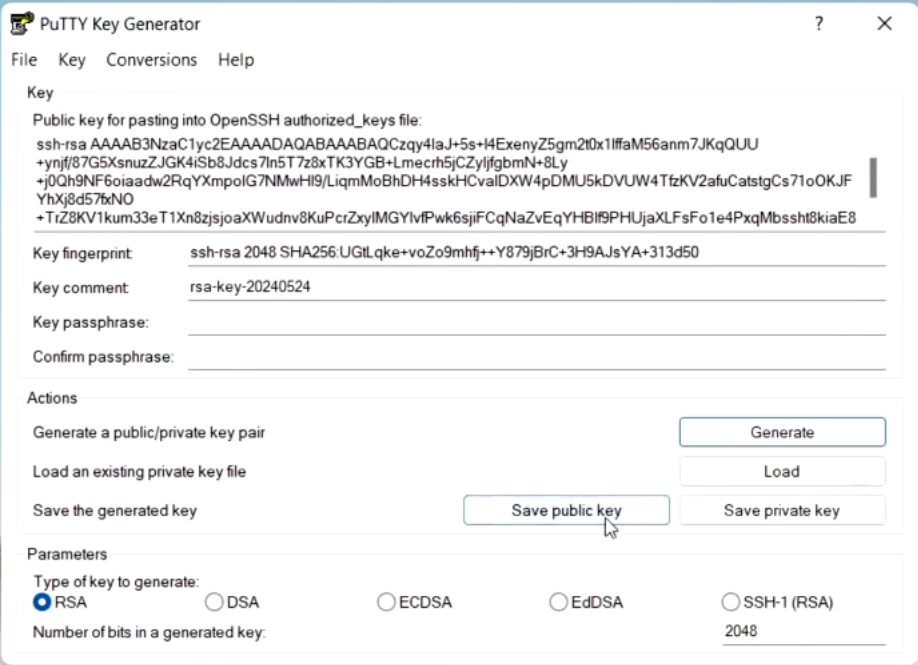
\includegraphics[width=0.8\linewidth,keepaspectratio]{figures/image-03.png}
\caption{Saving the generated public and private keys.}
\label{fig:save-ssh-keys}
\end{figure}
  \item Open PuTTY and select the private key file as shown in Figure~\ref{fig:putty-private-key}.
\begin{figure}[!htbp]
\centering
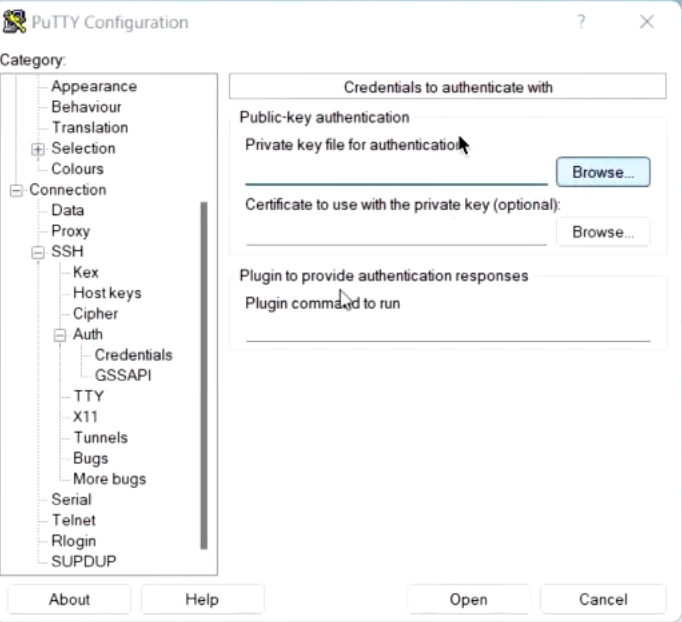
\includegraphics[width=0.8\linewidth,keepaspectratio]{figures/image-04.png}
\caption{Selecting a private key in PuTTY.}
\label{fig:putty-private-key}
\end{figure}
\FloatBarrier
\end{enumerate}



\subsection{Generate a Key in a Terminal}
\label{subsubsec:generate-terminal}
Open a terminal and run the following command:
  \begin{lstlisting}[style=terminal]
ssh-keygen -t rsa -b 4096 -f ~/.ssh/id_rsa_cuaim -C "abc@example.com"
\end{lstlisting}

This command creates a 4096-bit RSA key pair. The private key is stored at the specified path, and the public key is stored at the same path with the suffix \texttt{.pub}. The email address is only a label for identifying the key. When prompted, enter a passphrase to protect the private key.

\section{Request Account Authorization}
\label{subsec:authorize-ssh-key}

Send only the public key file, normally the file ending in \texttt{.pub}, to your professor or designated cluster contact. Wait for confirmation that the key has been added to your CU-AIM account before connecting.

\section{Optional: Transfer Files with Cyberduck}
\label{sec:cyberduck}
Cyberduck provides a graphical interface for transferring files on Windows and macOS. It is optional because files can also be managed through a terminal or VS Code. Install it from \url{https://cyberduck.io/download/}; the walkthrough video at \url{https://youtu.be/atx3VhDUOr8} shows the CU-AIM configuration.

Open Cyberduck, click the ``+'' button, enter the assigned server details, and select your SSH private key as shown in Figure~\ref{fig:cyberduck-settings}.

\begin{figure}[!htbp]
\centering
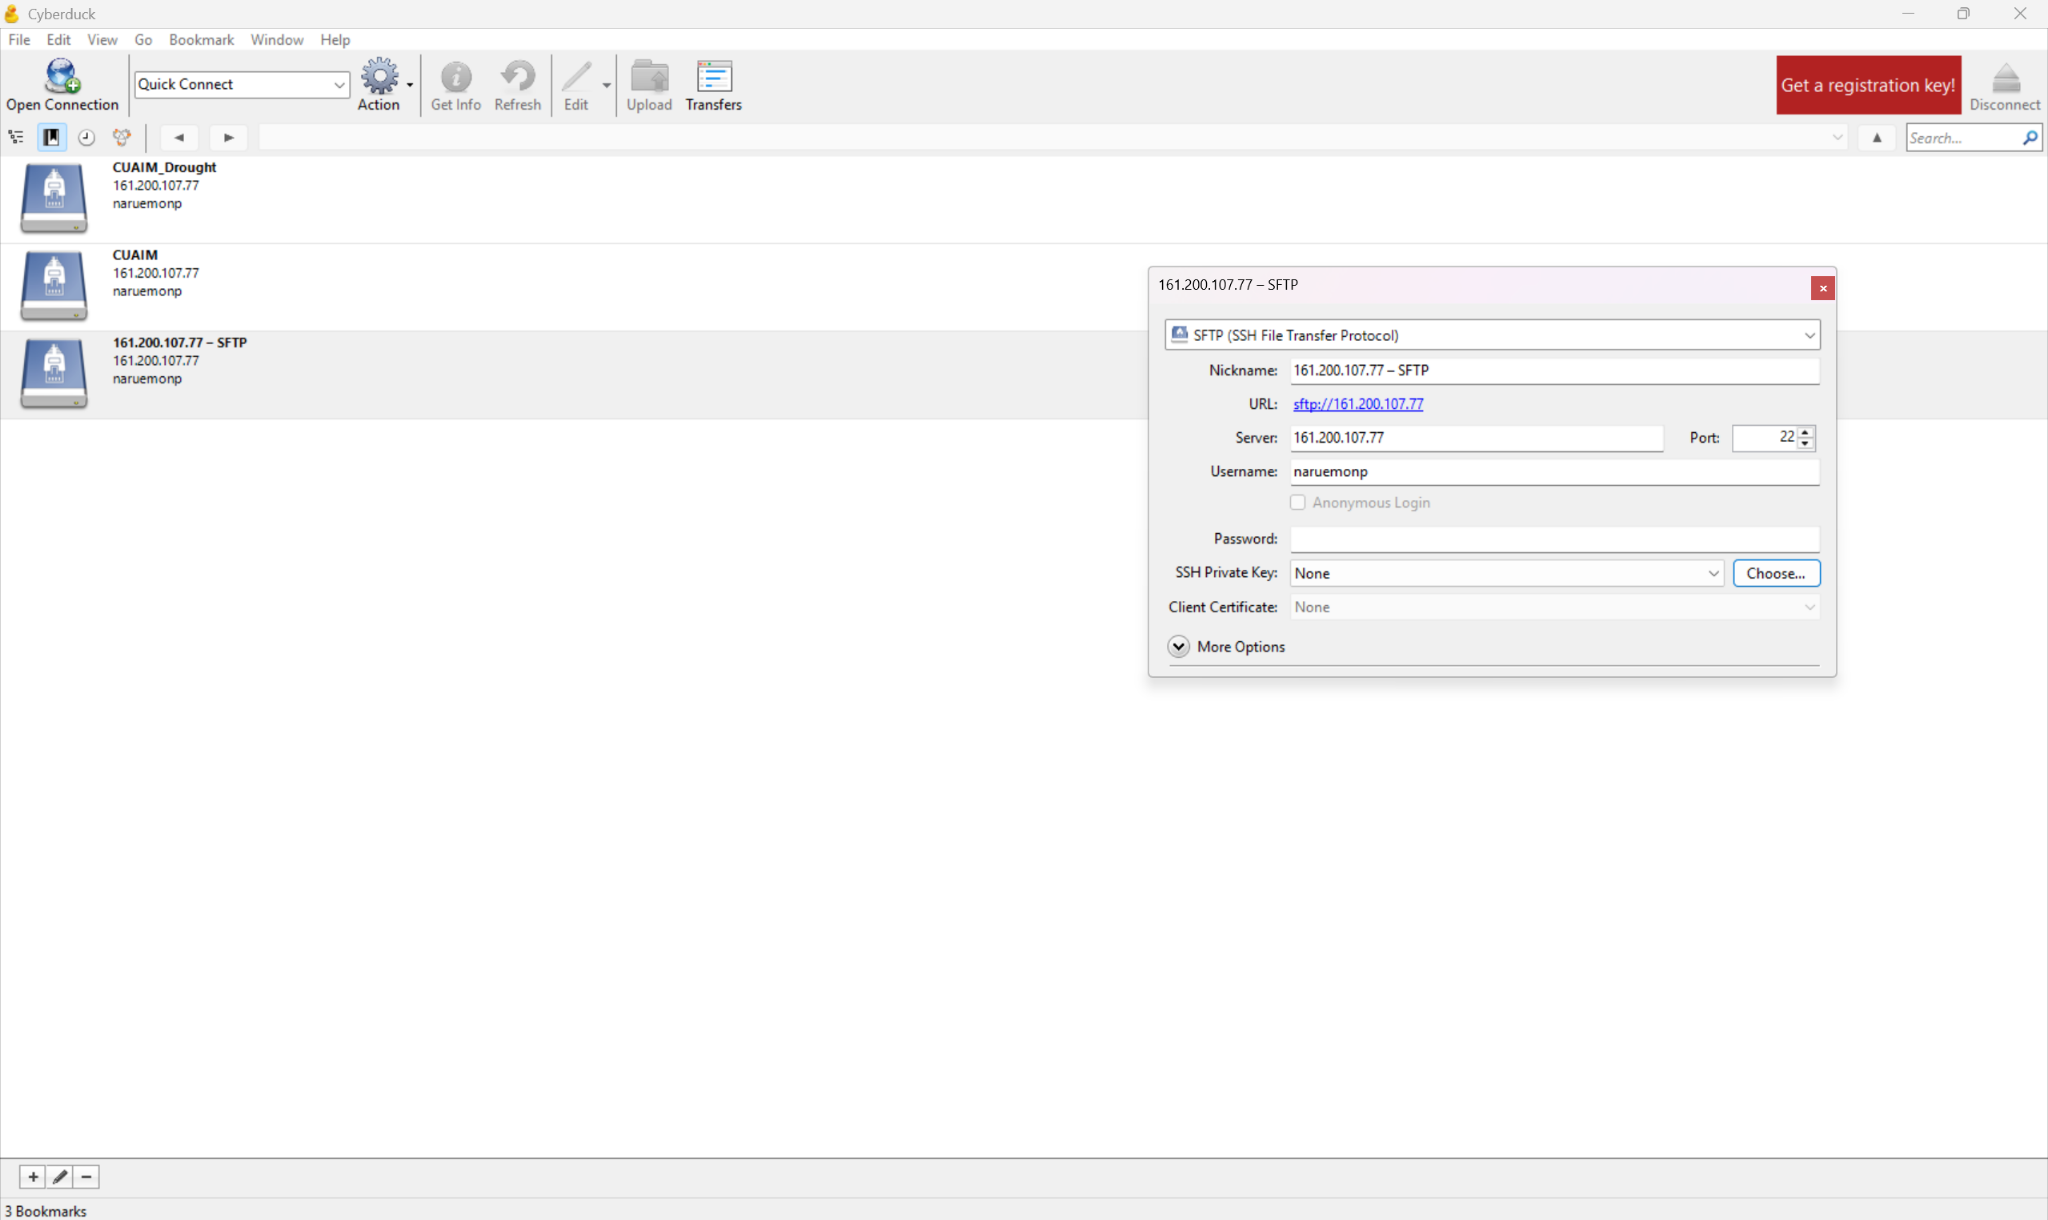
\includegraphics[width=\linewidth,height=0.78\textheight,keepaspectratio]{figures/image-05.png}
\caption{Cyberduck connection settings.}
\label{fig:cyberduck-settings}
\end{figure}

After connecting, open your assigned project directory. \textbf{Do not assume that \url{/data/home} is suitable for project data} because it may have a small storage quota. Confirm the correct path with your supervisor. Cyberduck is convenient for occasional drag-and-drop transfers; a terminal or VS Code is generally more efficient for repeated or large transfers.


\chapter{Connect to CU-AIM}
\label{chap:access-server}

Each work session begins by connecting to the Chula VPN as described in Section~\ref{sec:connect-vpn}. Keep the SSH private key on your local computer and confirm that your public key has been authorized.

\section{Connect from a Terminal}
\label{sec:terminal-ssh}
Open a local terminal and use SSH to connect:
  \begin{lstlisting}[style=terminal]
ssh naruemonp@161.200.107.77 -i </path/to/your/private_key>
\end{lstlisting}
A successful connection opens a shell on a CU-AIM login node. This entry computer is intended for file management, software setup, and Slurm submission commands. Submit computational work to Slurm instead of running it directly on the login node. Enter \texttt{exit} or \texttt{Ctrl + D} when you are ready to close the session. If the connection fails, first confirm the VPN connection, server address, username, key path, and account authorization.

\section{Install a Compatible VS Code Version}
\label{sec:download-vscode}

VS Code with the Remote-SSH extension provides a graphical editor and terminal for remote work. However, the current version of VS Code cannot be used with the CUAIM server because of incompatibilities with the system libraries on CU-AIM.

\begin{enumerate}
\item \href{https://vscode.download.prss.microsoft.com/dbazure/download/stable/8b3775030ed1a69b13e4f4c628c612102e30a681/VSCode-win32-x64-1.85.2.zip}
     {Download VS Code 1.85.2}

Fortunately, you do not need to uninstall your current version. Instead, download the compatible version above, extract the archive, and run \texttt{Code.exe} from the extracted directory whenever you need to access the CUAIM server. This release is older than the current version, so some recent extensions may not support it. You should also disable automatic updates for this installation and keep a separate, up-to-date installation for other work.

\begin{figure}[!htbp]
\centering
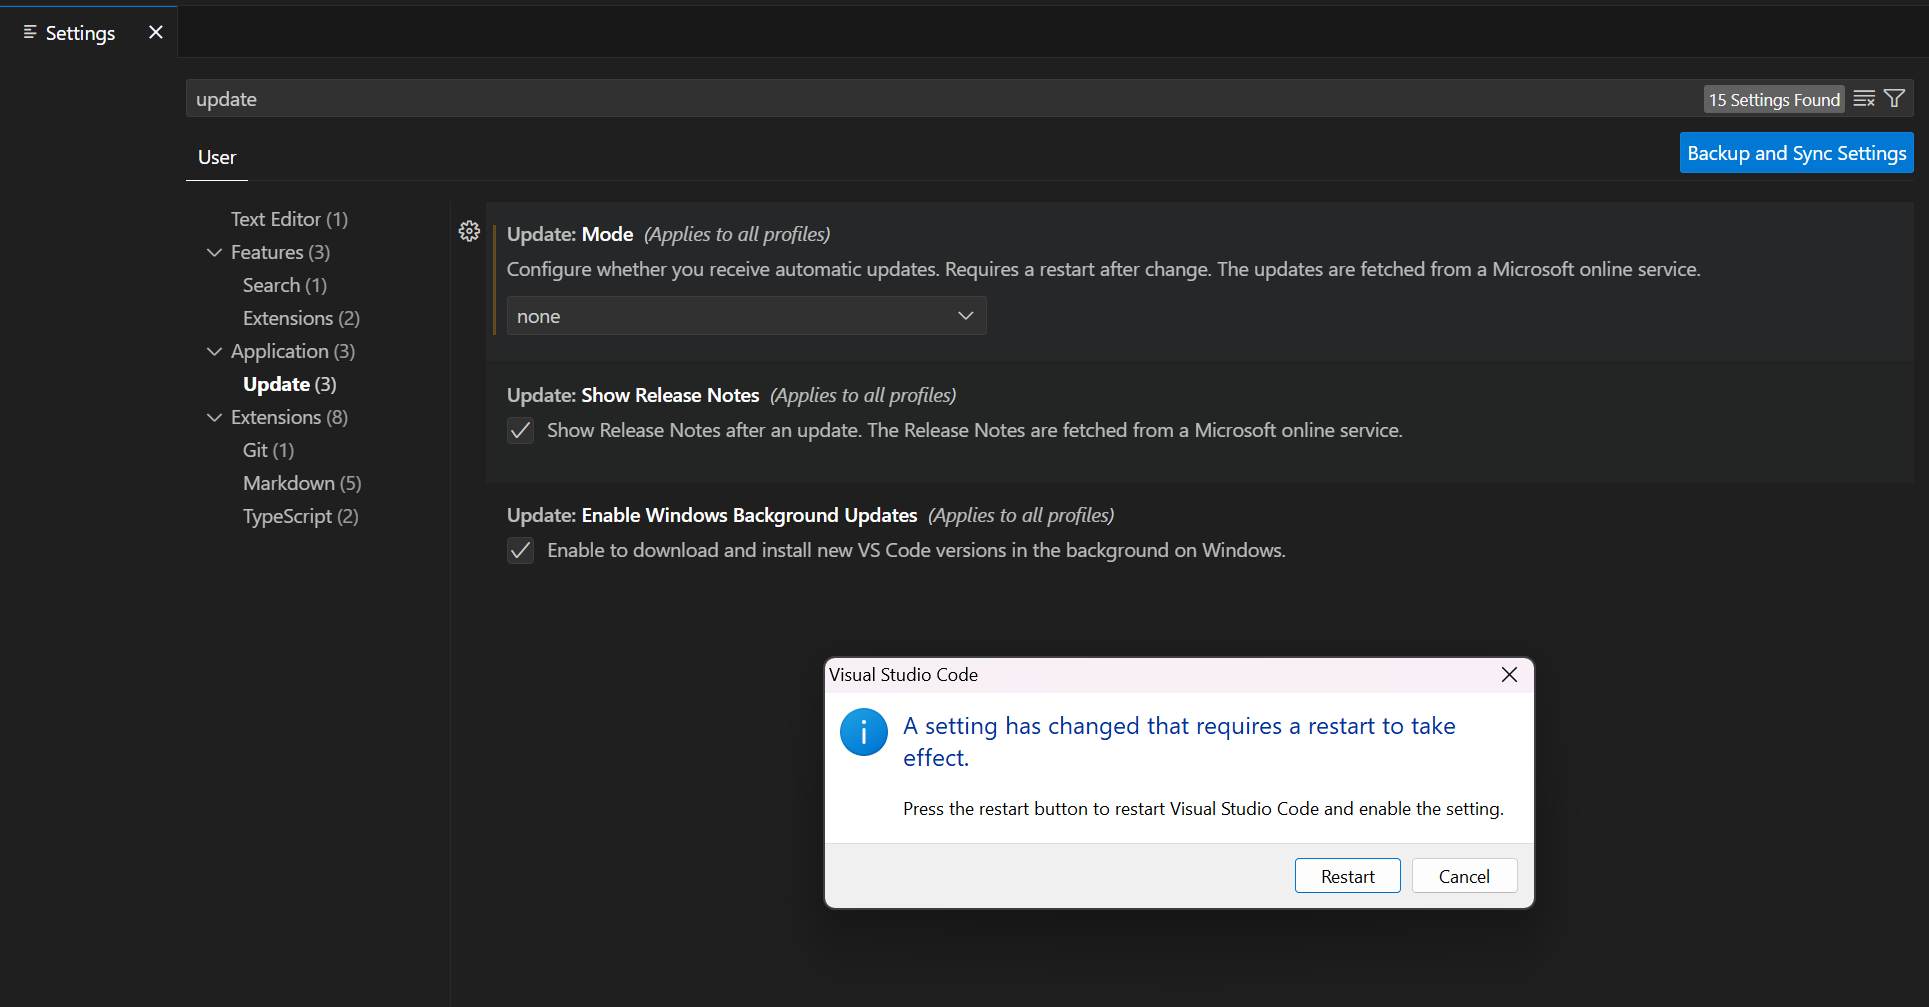
\includegraphics[width=\linewidth,height=0.78\textheight,keepaspectratio]{figures/image-06.png}
\caption{Disabling automatic updates in the tested VS Code installation.}
\label{fig:disable-vscode-updates}
\end{figure}

\item Then, install the \textbf{Remote-SSH} extension in this VS Code installation. If it does not load, install an extension version that supports the tested VS Code release.

\begin{figure}[!htbp]
\centering

\includegraphics[width=\linewidth,height=0.78\textheight,keepaspectratio]{figures/remote_ssh.png}
\caption{The Remote-SSH extension in VS Code.}
\label{fig:remote-ssh-extension}
\end{figure}
\end{enumerate}
\section{Configure Remote-SSH in VS Code}
\label{sec:configure-ssh-vscode}
\begin{enumerate}
  \item Open VS Code, press \textbf{Ctrl+Shift+P}, and select \textbf{Remote-SSH: Open SSH Configuration File}. Choose the user configuration file, normally \texttt{\%USERPROFILE\%/.ssh/config} on Windows.
  \item Add a host entry and replace each placeholder with your assigned value:
  \begin{lstlisting}
    
  Host cuaim
    HostName 161.200.107.77
    User naruemonp
    IdentityFile /path/to/your/private_key

  \end{lstlisting}
\end{enumerate}

To connect, press \textbf{Ctrl+Shift+P}, select \textbf{Remote-SSH: Connect to Host}, choose \texttt{cuaim}, and select \textbf{Linux} if prompted. A new VS Code window will open for the remote session. The next chapter explains how to open the correct project directory.
%%%%%%%%%%%%%%%%%%


\chapter{Plan Project Storage and Resources}
\label{chap:server-resources}
Before running a program, open the correct project directory and identify the resources that your account is permitted to request. This prevents common problems such as exceeding a storage quota or submitting a job with an unavailable QoS.

\section{Use the Assigned Project Directory}
\label{sec:access-folder}

After connecting, your session may begin in \url{/data/home/}. This home directory is suitable for small personal configuration files but may have limited storage. In VS Code, select \textbf{File $>$ Open Folder} and enter your assigned project path, for example:
\begin{lstlisting}
/data/project/your_project
\end{lstlisting}

Create a personal project folder within the assigned directory. If your research group has not specified a convention, use a descriptive name such as:
\begin{lstlisting}
{firstname}_{first character of the surname}_{project_name}
\end{lstlisting}

Keep source code, data, environments, model outputs, and logs within the approved project storage. Do not place large project files in \url{/data/home/}.

\section{Check Account and Scheduling Limits}
\label{sec:check-user-resources}
CU-AIM uses Slurm to assign computing resources. A \emph{Quality of Service} (QoS) is a named policy that can limit requested CPUs, GPUs, memory, and running time. A partition is a group of compute nodes used for a particular class of work. Your account must be allowed to use both the requested partition and QoS.

\subsection{Check the Available QoS Options}
\label{subsec:checking-resources}
\label{subsubsec:qos}
Run the CU-AIM helper command in a remote terminal:
\begin{lstlisting}[style=terminal]
  check_qos
\end{lstlisting}

\begin{figure}[!htbp]
\centering
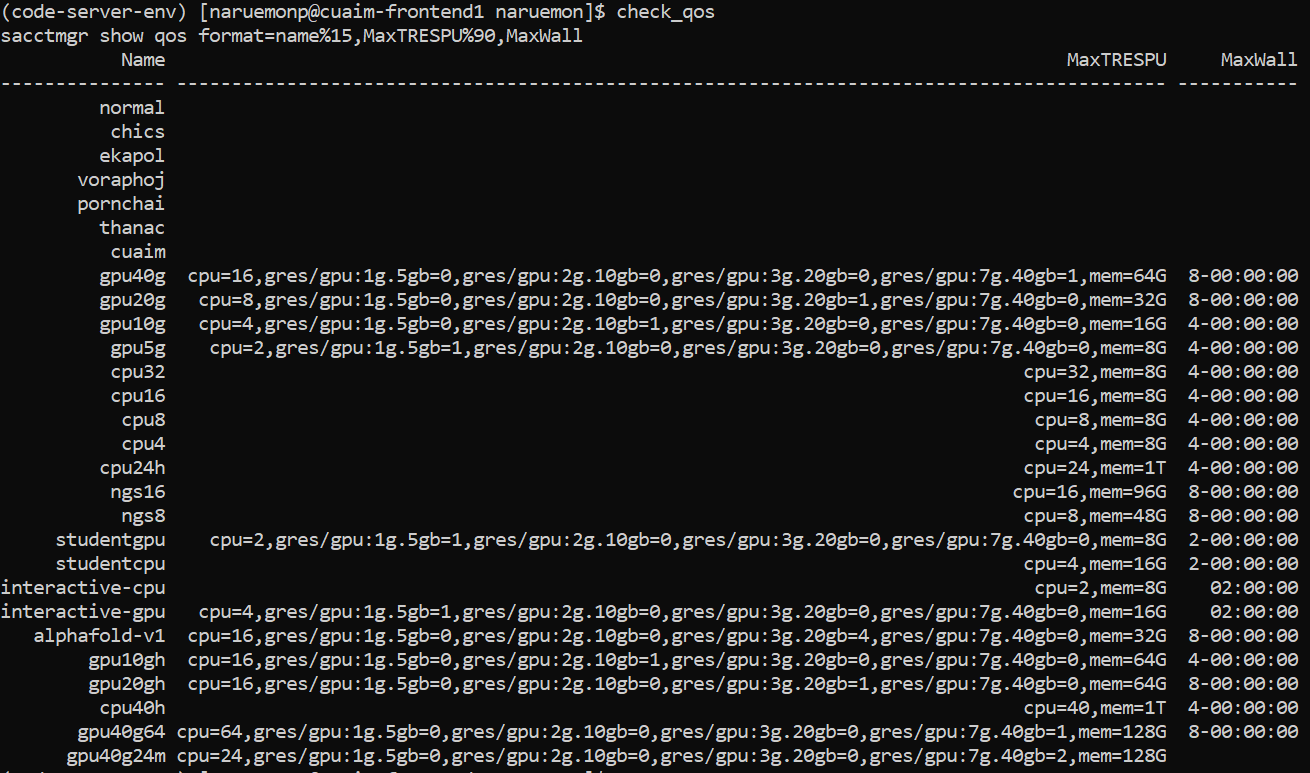
\includegraphics[width=\linewidth,height=0.78\textheight,keepaspectratio]{figures/image-11.png}
\caption{Example QoS information displayed by CU-AIM.}
\label{fig:qos-information}
\end{figure}

The output shows the QoS options and limits currently available to your account. Use this output as the authoritative source when it differs from this manual.

\FloatBarrier
\subsection{Check the Account Association}
\label{subsubsec:group-resources}

Access may also depend on your research group or Slurm account. Display the group information assigned to your user:
\begin{lstlisting}[style=terminal]
  check_group
\end{lstlisting}

Table~\ref{tab:qos-resources} records the QoS values available when this manual was prepared. These cluster settings may change, so verify them before every resource-intensive submission.
\begin{table}[!htbp]
\centering
\caption{Documented CU-AIM QoS limits}
\label{tab:qos-resources}
\begin{tabular}{lcccc}
\toprule
\textbf{QoS} & \textbf{CPUs} & \textbf{GPU resource} & \textbf{Memory} & \textbf{Maximum duration} \\
\midrule
\texttt{cpu40h} &
40 CPUs &
CPU only &
1 TB &
4 days \\

\texttt{interactive-gpu} &
4 CPUs &
1 $\times$ 1g.5gb &
16 GB &
2 hours \\

\texttt{gpu10gh} &
16 CPUs &
1 $\times$ 2g.10gb &
64 GB &
4 days \\

\texttt{gpu20gh} &
16 CPUs &
1 $\times$ 3g.20gb &
64 GB &
8 days \\

\texttt{gpu40g} &
16 CPUs &
1 $\times$ 7g.40gb &
64 GB &
8 days \\

\texttt{gpu40g24m} &
24 CPUs &
2 $\times$ 7g.40gb &
128 GB &
8 days \\
\bottomrule
\end{tabular}
\end{table}

The following standard Slurm accounting command provides another view of the account and QoS associations for a user:
\begin{lstlisting}[style=terminal]
  sacctmgr show assoc user=naruemonp format=account,user%15,qos%50
\end{lstlisting}


\section{Inspect Partitions and Compute Nodes}
\label{subsec:nodes-partitions}
The scheduler runs jobs on compute nodes within a partition. Use \texttt{sinfo} to inspect node states and advertised resources:
\begin{lstlisting}[style=terminal]
sinfo -o "%.15R %.8D %.10m %.5c %7z %60G %N"
\end{lstlisting}

\begin{figure}[!htbp]
\centering
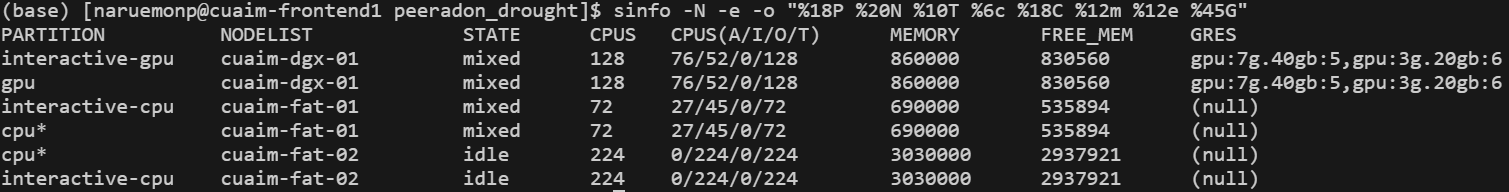
\includegraphics[width=\linewidth,height=0.78\textheight,keepaspectratio]{figures/sinfo_2.png}
\caption{Example Slurm node and partition information.}
\label{fig:sinfo-node-information}
\end{figure}
The output summarizes partitions, node states, memory, CPUs, and configured resources. To inspect one node in more detail, use:
\begin{lstlisting}[style=terminal]
scontrol show node <node-name>
\end{lstlisting}
\begin{figure}[!htbp]
\centering
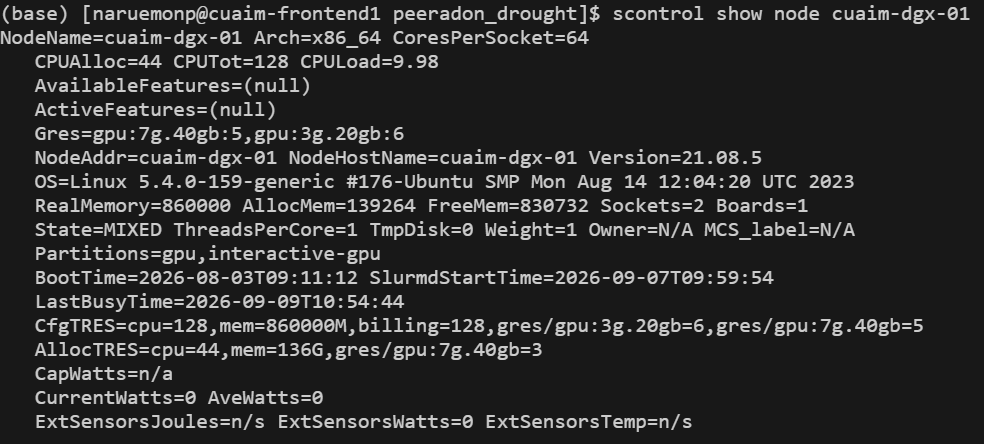
\includegraphics[width=\linewidth,height=0.78\textheight,keepaspectratio]{figures/scontrol.png}
\caption{Detailed information for a Slurm node.}
\label{fig:scontrol-node-information}
\end{figure}

Do not request a particular node unless the CU-AIM documentation or a cluster administrator instructs you to do so. A narrow node request can keep an otherwise valid job waiting in the queue. Chapter~\ref{chap:run-slurm-jobs} explains how to inspect a pending job.

\chapter{Run and Monitor Slurm Jobs}
\label{chap:run-slurm-jobs}
\section{Understand a Slurm Job}
\label{sec:jobs}
A Slurm job combines a request for resources with one or more commands to run. The requested resources form a job allocation. If the allocation is not immediately available, Slurm keeps the job pending in a queue. When resources become available, the job runs on one or more compute nodes.

Before submitting a job, confirm the permitted QoS and partition, estimate the required CPUs, GPUs, memory, and duration, and prepare the software environment described in Section~\ref{sec:software-modules}. Request only what the program needs because larger requests can wait longer for a suitable node.

\section{Choose a Submission Method}
\label{sec:job-submissions}
Use an interactive job for short experiments and troubleshooting. Use a batch job for routine analyses, training runs, or any work that should continue without an open terminal.

\subsection{Start an Interactive Job with \texttt{srun}}
\label{subsec:interactive-srun}

Run \texttt{srun} from a remote terminal to request resources and open an interactive shell. The command may wait until the scheduler can satisfy the request. Once it starts, the terminal is attached to the allocated compute node. If \texttt{srun} is called within an existing allocation, it starts a job step inside that allocation instead of creating another allocation.

\begin{lstlisting}[style = terminal]
srun -p gpu -c2 --mem=8G --qos=gpu40g --gres=gpu:7g.40gb:1 --pty bash -l
\end{lstlisting}
\begin{table}[ht]
\centering
\begin{tabular}{|l|p{10cm}|}
\hline
\textbf{Option} & \textbf{Description} \\ \hline

\texttt{--qos=gpu40g24m} &
Selects the QoS for the request. Use only a QoS available to your account. \\ \hline

\texttt{-c2} &
Requests two CPU cores for the task. \\ \hline

\texttt{--mem=8G} &
Requests 8 GB of memory for the job. \\ \hline

\texttt{-p gpu} &
Selects the GPU partition. The partition and QoS must be compatible. \\ \hline

\texttt{--gres=gpu:7g.40gb:1} &
Requests one GPU resource with the specified profile. Use a profile listed by CU-AIM. \\ \hline

\texttt{--pty bash -l} &
Starts an interactive login shell after the resources are allocated. \\ \hline

\end{tabular}
\caption{Options used in the interactive job example}
\label{tab:job-submission-options}
\end{table}

To finish, run \texttt{exit} or press \textbf{Ctrl+D}. Confirm with \texttt{squeue -u your\_username} that the job has ended and its resources have been released.


\subsection{Submit a Batch Job with \texttt{sbatch}}
\label{subsec:batch-sbatch}

The \texttt{sbatch} command submits a shell script, commonly saved with a \texttt{.sh} extension. Lines beginning with \texttt{\#SBATCH} describe the requested resources and log files. Other lines prepare the environment and run the program. After submission, Slurm returns a job ID. Record this ID because it identifies the job in queue, accounting, log, and cancellation commands. Immediately afterward, the terminal returns, and the script starts automatically when resources become available.

The following template shows the structure of a GPU batch job. It contains both a Python-script command and a notebook command for illustration. Retain only the command required by your own job when you create a working script.
\begin{lstlisting}[language=Python]
#!/bin/bash -l

#SBATCH --job-name=mtj
#SBATCH --partition=gpu
#SBATCH --qos=gpu40g
#SBATCH --gres=gpu:7g.40gb:1
#SBATCH --mem=20G
#SBATCH --cpus-per-task=2
#SBATCH --output=mtj-%j.out
#SBATCH --error=mtj-%j.err
#SBATCH --time=24:00:00     

mkdir -p logs
module load Anaconda3
module load CUDA/11.8.0
eval "$(conda shell.bash hook)"
conda activate my_project

srun --output=logs/script1-%j.out \
     --error=logs/script1-%j.err \
     python -u script1.py



# if you want to execute .ipynb makesure you install papermill library first
srun --output=logs/script1-%j.out \
     --error=logs/script1-%j.err \
     papermill input.ipynb outputs/executed_output.ipynb
  
# srun allows Slurm to manage the job step and resource binding.
# This makes it easier to run jobs with multiple tasks, MPI, or multiple nodes.

echo "Job completed at $(date)"
exit $?
\end{lstlisting}

Submit the script from a login-node terminal. Do not have to start an interactive allocation first.
\begin{lstlisting}
  sbatch <file_name>.sh
\end{lstlisting}
Before submission, check the following items:
\begin{itemize}
  \item The partition, QoS, GPU profile, memory, CPU count, and time comply with current limits.
  \item Each \texttt{\#SBATCH} directive uses a valid Slurm option for CU-AIM.
  \item The script loads only the required modules and activates the intended Python environment.
  \item Input paths exist, and the output and error paths point to writable project storage.
  \item The requested working directory is correct. By default, a batch job begins in the directory from which \texttt{sbatch} was called.
\end{itemize}

\begin{figure}[!htbp]
\centering
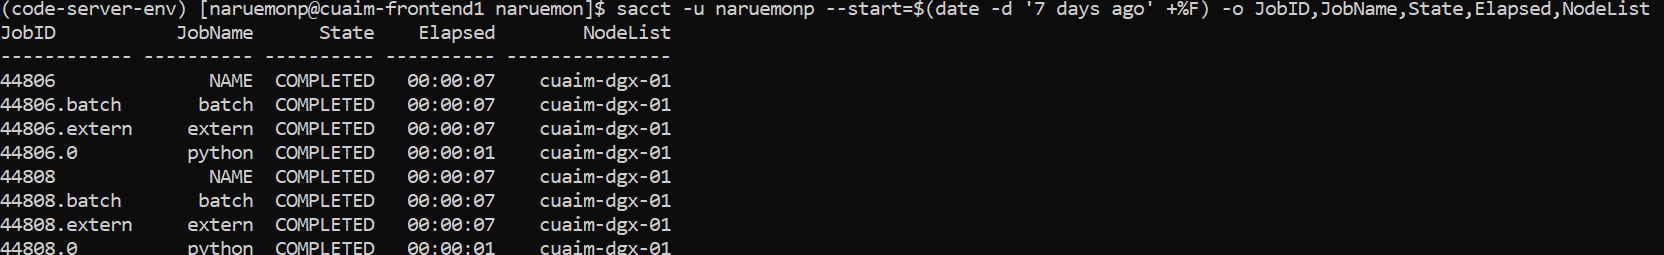
\includegraphics[width=\linewidth,height=0.78\textheight,keepaspectratio]{figures/image-16.png}
\caption{Example batch-job monitoring information.}
\label{fig:batch-job-monitoring}
\end{figure}


Section~\ref{sec:monitoring-queue} explains how to monitor the submitted job. For multiple workloads, request the resources required by each job and respect any aggregate limits on the user, group, account, partition, or QoS. Section~\ref{subsec:resource-sharing} discusses this case.


\section{Cancel a Job}
\label{subsec:cancel-jobs}
Standard Slurm cancels one or more jobs with \texttt{scancel} followed by their job IDs. The \texttt{-f} ensures the entire job is stopped, including the batch script/shell and all running job steps or subprocesses launched by it.
\begin{lstlisting}
   scancel-f <JOB_ID01> <JOB_ID02> <JOB_ID03>
\end{lstlisting}



\section{Prepare the Software Environment}
\label{sec:software-modules}

Each job needs a defined set of software and libraries. CU-AIM provides shared software through environment modules. Loading a module makes a particular version of Python, CUDA, or another program available in the current shell without changing the system installation.

\subsection{Inspect and Load Environment Modules}
\label{subsec:environment-modules}

Use these commands to inspect and manage modules:

\begin{lstlisting}[style=terminal]
module avail                    # List available modules
module spider <module-name>     # Search for a specific module
module load <module-name>       # Load a module
module list                     # Show currently loaded modules
module unload <module-name>     # Unload a module
module purge                    # Unload all modules
\end{lstlisting}

For example, the following commands prepare Anaconda and a CUDA toolkit in the current shell:

\begin{lstlisting}[style=terminal]
module purge
module load Anaconda3
module load CUDA/11.8.0
module list
\end{lstlisting}

Please record the module names and versions used by the project and load the same compatible set when installing packages and running jobs.

\subsection{Check GPU and CUDA Compatibility}
\label{subsec:checking-cuda}
GPU software depends on the GPU model, NVIDIA driver, CUDA toolkit or runtime, and the machine-learning framework. After obtaining a GPU allocation, inspect the GPU and driver:
\begin{lstlisting}[style = terminal]
  nvidia-smi
\end{lstlisting}
\begin{figure}[!htbp]
  \centering
  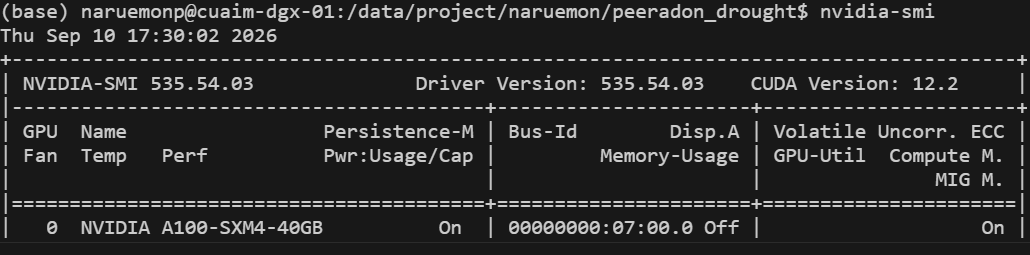
\includegraphics[width=\linewidth,height=0.78\textheight,keepaspectratio]{figures/nvidia-smi.png}
\caption{Example GPU and NVIDIA driver information reported by \texttt{nvidia-smi}.}
  \label{fig:nvidia-smi}
\end{figure}
The CUDA version shown by \texttt{nvidia-smi} indicates the newest CUDA version supported by the installed driver.

\FloatBarrier
\subsection{Create a Conda Environment}
\label{subsec:conda-environment}

Install project-specific Python libraries in a separate Conda environment instead of the system Python installation. After loading Anaconda and any required CUDA module, create and activate an environment:

\begin{lstlisting}[style=terminal]
module load Anaconda3
module load CUDA/11.8.0
eval "$(conda shell.bash hook)"
conda create -n my_project python=3.11
conda activate my_project
\end{lstlisting}

If \texttt{conda activate} is unavailable in the current shell, initialize the Conda shell function and try again:

\begin{lstlisting}[style=terminal]
eval "$(conda shell.bash hook)"
conda activate my_project
\end{lstlisting}

\subsection{Use a Python Virtual Environment}
\label{subsec:python-venv}

A Python virtual environment, or \texttt{venv}, is a lighter alternative when the required Python module is available:

\begin{lstlisting}[style=terminal]
python -m venv ~/venvs/my_project
source ~/venvs/my_project/bin/activate
python -m pip install --upgrade pip
python -m pip install numpy pandas scikit-learn
\end{lstlisting}

Conda and \texttt{venv} are alternatives. Choose one for each project and document the environment so that another student can reproduce it.

\subsection{Activate the Environment in a Batch Job}
\label{subsec:batch-environment}

A batch job starts in a new, non-interactive shell. It does not reliably inherit the software configuration of a previous terminal session. Therefore, a user have to load the required modules and activate the project environment in every job script:

\begin{lstlisting}[language=bash, caption={example\_batch\_job.sh}]
#!/bin/bash -l
#SBATCH --job-name=my_project
#SBATCH --output=logs/my_project-%j.out
#SBATCH --error=logs/my_project-%j.err
#SBATCH --partition=gpu
#SBATCH --qos=<qos>
#SBATCH --gres=gpu:1
#SBATCH --cpus=4
#SBATCH --mem=16G
#SBATCH --time=04:00:00

cd "$SLURM_SUBMIT_DIR"

module purge
module load Anaconda3
module load CUDA/11.8.0

eval "$(conda shell.bash hook)"
conda activate my_project

which python
python --version
python my_script.py
\end{lstlisting}


\section{Monitor Jobs and the Queue}
\label{sec:monitoring-queue}
To monitor their pending job, the user can use \texttt{squeue} while a job is pending, running, or finished.

\subsection{Inspect Pending and Running Jobs}
The following format displays the job ID, partition, name, user, state, elapsed time, time limit, node count, pending reason or node list, and GPU information:

\begin{lstlisting}
squeue -o "%.18i %.9P %.8j %.8u %.8T %.10M %.9l %.6D %R %b"
\end{lstlisting}

The full display may include other users' jobs that your account is permitted to view.

\begin{figure}[!htbp]
\centering
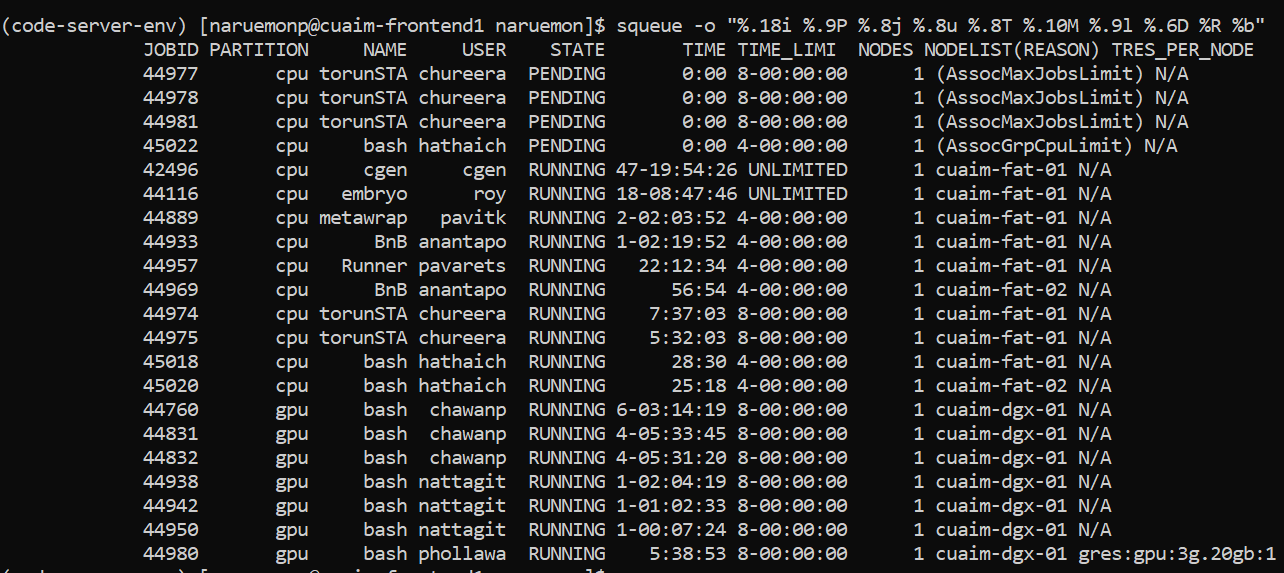
\includegraphics[width=\linewidth,height=0.78\textheight,keepaspectratio]{figures/image-14.png}
\caption{Example Slurm queue information.}
\label{fig:squeue-information}
\end{figure}

\begin{lstlisting}
squeue -u naruemonp
\end{lstlisting}

Replace the placeholder to show only your jobs. For a pending job, read the reason in the final output column before changing the request. Common reasons include unavailable resources, priority, account limits, or a dependency on another job. Do not attempt to cancel another user's job; contact a cluster administrator if intervention is required.

\FloatBarrier
\subsection{Inspect Job Results}
Use the job ID returned by \texttt{sbatch} to inspect the final state and exit code:

\begin{lstlisting}
sacct -j <job_id> --format=JobID,JobName,State,ExitCode,Elapsed
\end{lstlisting}

An exit code of \texttt{0:0} usually indicates that the batch script completed successfully. A nonzero exit code means that the script or one of its commands failed. Read the job's output and error files to identify the cause.

\begin{figure}[!htbp]
\centering
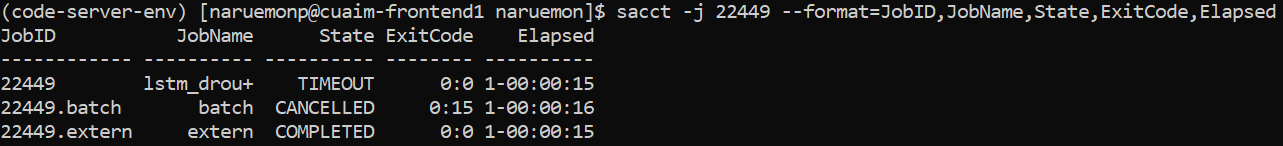
\includegraphics[width=\linewidth,height=0.78\textheight,keepaspectratio]{figures/image-15.png}
\caption{Example Slurm accounting information for a job.}
\label{fig:sacct-job-information}
\end{figure}

Queue and accounting output commonly includes these fields:
\begin{description}

\item[\textbf{JOBID}] The unique job identifier.

\item[\textbf{PARTITION}] The requested compute partition.

\item[\textbf{NAME}] The name assigned in the submission command or script.

\item[\textbf{USER}] The user running the job.

\item[\textbf{ST}] The current state code, summarized in Table~\ref{tab:job-status}.

\item[\textbf{TIME}] The elapsed running time. A pending job normally displays zero.

\item[\textbf{NODES}] The number of allocated or requested compute nodes.

\item[\textbf{NODELIST}] The allocated node names for a running job, or the waiting reason for a pending job.

\end{description}

\begin{table}[ht]
\centering
\caption{Slurm job status codes}
\label{tab:job-status}
\begin{tabularx}{\textwidth}{l l X}
\toprule
\textbf{Status} & \textbf{Code} & \textbf{Explanation} \\
\midrule
COMPLETED  & CD & The job finished successfully. \\
COMPLETING & CG & The job has stopped running and Slurm is releasing its resources. \\
FAILED     & F  & The job ended with an error or nonzero exit code. \\
PENDING    & PD & The job is waiting for scheduling conditions to be satisfied. \\
RUNNING    & R  & The job has resources and is executing. \\
\bottomrule
\end{tabularx}
\end{table}

\begin{lstlisting}
sacct -u naruemonp --start=$(date -d '7 days ago' +%F) -o JobID,JobName,State,Elapsed,NodeList
\end{lstlisting}

This command lists jobs recorded for the specified user during the previous seven days. Use it to find completed, failed, canceled, or time-limited jobs when the job ID is not known.

\begin{figure}[!htbp]
\centering
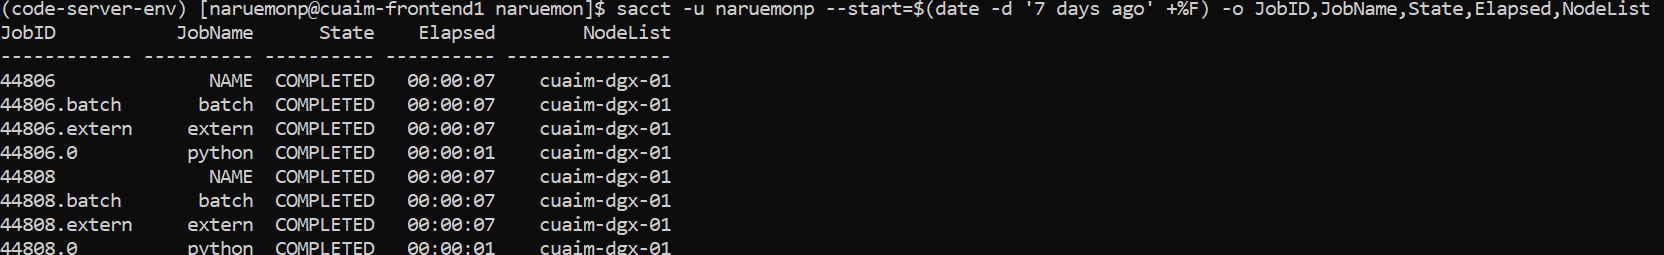
\includegraphics[width=\linewidth,height=0.78\textheight,keepaspectratio]{figures/image-16.png}
\caption{Example accounting information for completed jobs.}
\label{fig:completed-job-information}
\end{figure}

If the available QoS or project storage does not meet a documented research requirement, contact your supervisor or the cluster administrator. Include the expected CPU, GPU, memory, storage, and duration requirements so that the request can be evaluated.


\chapter{Coordinate Multiple Slurm Workloads}
\label{chap:advanced-slurm}
This chapter is optional for first-time users. Read it when a project must run several independent programs or a defined sequence of programs. Begin with separate batch jobs unless the programs must share one allocation or run in a strict order.

\section{Distinguish Jobs, Tasks, and Job Steps}
\label{sec:resource-allocation}

\subsection{Core Definitions}
\label{subsec:jobs-tasks}
The following terms describe how Slurm organizes work:
\begin{itemize}
    \item \textbf{Job}: A submitted resource request and its commands. The allocation may include CPUs, GPUs, memory, and a time limit.
    \item \textbf{Task}: A process within a job. One job may contain one or more tasks.
    \item \textbf{Job step}: A unit of work launched within an existing allocation, commonly with \texttt{srun}.
\end{itemize}

\subsection{Sharing Resources Between Workloads}
\label{subsec:resource-sharing}
Slurm may apply limits to each job and to the combined activity of a user, group, account, partition, or QoS. Request the resources needed by each workload and check the current aggregate limits. If a program exceeds its assigned memory, Slurm or the operating system may terminate it. Inspect the accounting record and error log after such a failure.

\section{Choose a Multi-Program Structure}
\label{subsec:workload-strategies}
Multiple programs can use separate allocations or share one allocation. The correct choice depends on whether they must be scheduled, monitored, and retried independently.

\subsection{Submit Independent Jobs}
\label{par:independent-jobs}
This approach gives each program its own job allocation. It is appropriate when the programs do not need to start together. Each job can be monitored, retried, or canceled independently.

\begin{lstlisting}[language=bash, caption={Sample for job1.sh}]
#!/bin/bash -l
#SBATCH --job-name=mtj01
#SBATCH --partition=gpu
#SBATCH --qos=gpu40g24m
#SBATCH --gres=gpu:7g.40gb:1
#SBATCH --mem=20G
#SBATCH --cpus-per-task=2
#SBATCH --output=mtj-%j.out
#SBATCH --error=mtj-%j.err
#SBATCH --time=24:00:00

python script1.py
\end{lstlisting}

\begin{lstlisting}[language=bash, caption={Sample for job2.sh}]
#!/bin/bash -l
#SBATCH --job-name=mtj02
#SBATCH --partition=gpu
#SBATCH --qos=gpu40g24m
#SBATCH --gres=gpu:7g.40gb:1
#SBATCH --mem=20G
#SBATCH --cpus-per-task=2
#SBATCH --output=mtj-%j.out
#SBATCH --error=mtj-%j.err
#SBATCH --time=24:00:00

python script2.py
\end{lstlisting}
Submit the scripts separately with \texttt{sbatch job1.sh} and \texttt{sbatch job2.sh}. Slurm schedules each job according to its request and the applicable limits.

\subsection{Run Concurrent Steps Within One Job}
\label{par:multiple-tasks}
This approach requests one allocation large enough for all programs. Each \texttt{srun} command starts a job step within that allocation. Use it only when the parent allocation provides the combined CPUs, memory, and GPUs required by all steps.

\begin{lstlisting}[language=bash, caption={combined\_job.sh}]
#!/bin/bash -l
#SBATCH --job-name=mtj
#SBATCH --partition=gpu
#SBATCH --qos=gpu40g24m
#SBATCH --gres=gpu:7g.40gb:2
#SBATCH --mem=20G
#SBATCH --cpus-per-task=2
#SBATCH --output=mtj-%j.out
#SBATCH --error=mtj-%j.err
mkdir -p logs

# Launch task 1 in the background
srun --exclusive \
     --ntasks=1 \
     --cpus-per-task=1 \
     --gres=gpu:7g.40gb:1 \
     --mem=10G \
     --output=logs/script1-%j.out \
     --error=logs/script1-%j.err \
     python -u script1.py &

pid1=$!

# Launch task 2 in the background
srun --exclusive \
     --ntasks=1 \
     --cpus-per-task=1 \
     --gres=gpu:7g.40gb:1 \
     --mem=10G \
     --output=logs/script2-%j.out \
     --error=logs/script2-%j.err \
     python -u script2.py &

pid2=$!

# Wait for both tasks and preserve their exit statuses
wait "$pid1"
status1=$?

wait "$pid2"
status2=$?

if [[ $status1 -ne 0 || $status2 -ne 0 ]]; then
    echo "At least one task failed."
    exit 1
fi

echo "Both tasks completed successfully."
\end{lstlisting}

The ampersand (\texttt{\&}) allows the two shell commands to overlap. Actual concurrent execution still depends on sufficient resources and valid Slurm step requests. The final \texttt{wait} commands keep the batch job active until both programs finish.


\section{Run a Numbered Series of Programs}
\label{sec:execution-loops}

Use a job array when numbered programs are independent. Use a shell loop within one batch job when they must run in a strict order. A concurrency limit on a job array controls how many elements run at once, but it does not guarantee numerical execution order.

\subsection{Limit a Job Array to One Running Element}
\label{subsec:job-array}

The following excerpt illustrates a ten-element array with a concurrency limit of one:

\begin{lstlisting}[language=bash,caption={The array and task-selection lines in \texttt{test\_sequential\_job.sh}}]
# Create ten array elements; at most one may run at a time.
#SBATCH --array=1-10%1

i="$SLURM_ARRAY_TASK_ID"
python -u "script${i}.py"
\end{lstlisting}

The range \texttt{1-10} creates ten array elements. The suffix \texttt{\%1} allows no more than one element to run at a time. Other elements remain pending until the running element finishes and all scheduling conditions are met. Slurm chooses which eligible element starts next, so this pattern must not be used when one program depends on the output of the previous index.

\begin{figure}[!htbp]
\centering
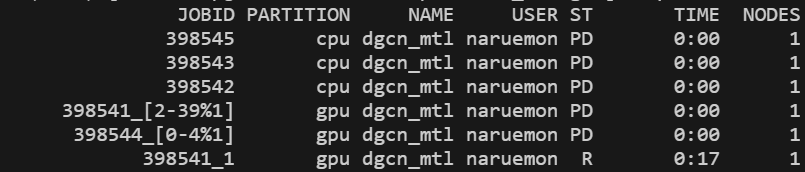
\includegraphics[width=\linewidth]{figures/slurm-sequential-array.png}
\caption{A Slurm queue showing a running array element and pending elements constrained by an array concurrency limit.}
\label{fig:slurm-sequential-array}
\end{figure}

The complete included example currently defines three array elements. Adjust its array range in a working copy to match the number of programs in your project:

\lstinputlisting[language=bash,caption={A Slurm job array with limited concurrency},label={lst:sequential-job}]{ssh_example/test_sequential_job.sh}

Each element receives a \texttt{SLURM\_ARRAY\_TASK\_ID}, which selects the corresponding program. The array job ID and element index in each log filename make the runs individually traceable.

\subsection{Run a Strict Sequence Within One Batch Job}
\label{subsec:single-job-loop}

The next example submits one batch job and loops through ten programs within the same allocation:

\lstinputlisting[language=bash,caption={A strict sequence within one batch job},label={lst:sequential-task}]{ssh_example/test_sequential_task.sh}

Each \texttt{srun} command finishes before the loop starts the next iteration, so the numerical order is preserved. The script uses shell error handling to stop after a failed step. All steps share the time limit of the parent allocation, so estimate the total duration of the complete sequence.

The two approaches can be summarized as follows:

\begin{table}[!htbp]
\centering
\caption{Comparison of numbered Slurm execution patterns}
\label{tab:sequential-slurm-patterns}
\begin{tabularx}{\textwidth}{l X X}
\toprule
\textbf{Property} & \textbf{Job array} & \textbf{Single job loop} \\
\midrule
Slurm records & One array with individually traceable elements & One batch job with several job steps \\
Execution order & Not guaranteed by the \texttt{\%1} concurrency limit & Preserved by the blocking \texttt{for} loop \\
Failure handling & Each element has its own state & The script can stop the loop after a failed step \\
Use when & Programs are independent & Programs must run in order within one allocation \\
\bottomrule
\end{tabularx}
\end{table}

Submit and monitor the array version with:

\begin{lstlisting}[language=bash]
sbatch ssh_example/test_sequential_job.sh
squeue -u "$USER"
\end{lstlisting}

Use the array version for independent programs that benefit from separate states and logs. Use the single-job loop when order matters or all programs must share one allocation.



\chapter{Use Singularity Containers}
\label{chap:containers}
Use a container only when the module and Python-environment workflow in Section~\ref{sec:software-modules} cannot provide compatible dependencies. A Singularity image is a file containing an isolated software environment. It can provide newer application libraries, but it still uses the host operating-system kernel and, for GPU work, the host NVIDIA driver.

\section{Obtain a Container Image}
\label{sec:download-container}
First confirm that Singularity is available on CU-AIM and that the selected image is permitted by cluster policy. The following commands download a Docker or Open Container Initiative (OCI) image and save it as a Singularity Image Format (SIF) file:
\begin{lstlisting}[style = terminal]

PROJECT=/data/project/naruemon/<project_name>

export SINGULARITY_CACHEDIR="$PROJECT/.singularity-cache-$USER"
export SINGULARITY_TMPDIR="$PROJECT/.singularity-tmp-$USER"
export TMPDIR="$PROJECT/tmp-$USER"

mkdir -p "$SINGULARITY_CACHEDIR" "$SINGULARITY_TMPDIR" "$TMPDIR"

singularity pull \
  "$PROJECT/<singularity_name>.sif" \
  docker://<pull_url>

singularity cache clean --force
\end{lstlisting}
The environment variables redirect download and temporary files from the limited home directory to project storage. The output path in \texttt{singularity pull} determines where the final SIF file is stored.

Use an image from a trusted registry. Record the registry address, image name, and immutable version or digest in the project documentation so that the environment can be reproduced.
\begin{figure}[!htbp]
  \centering
  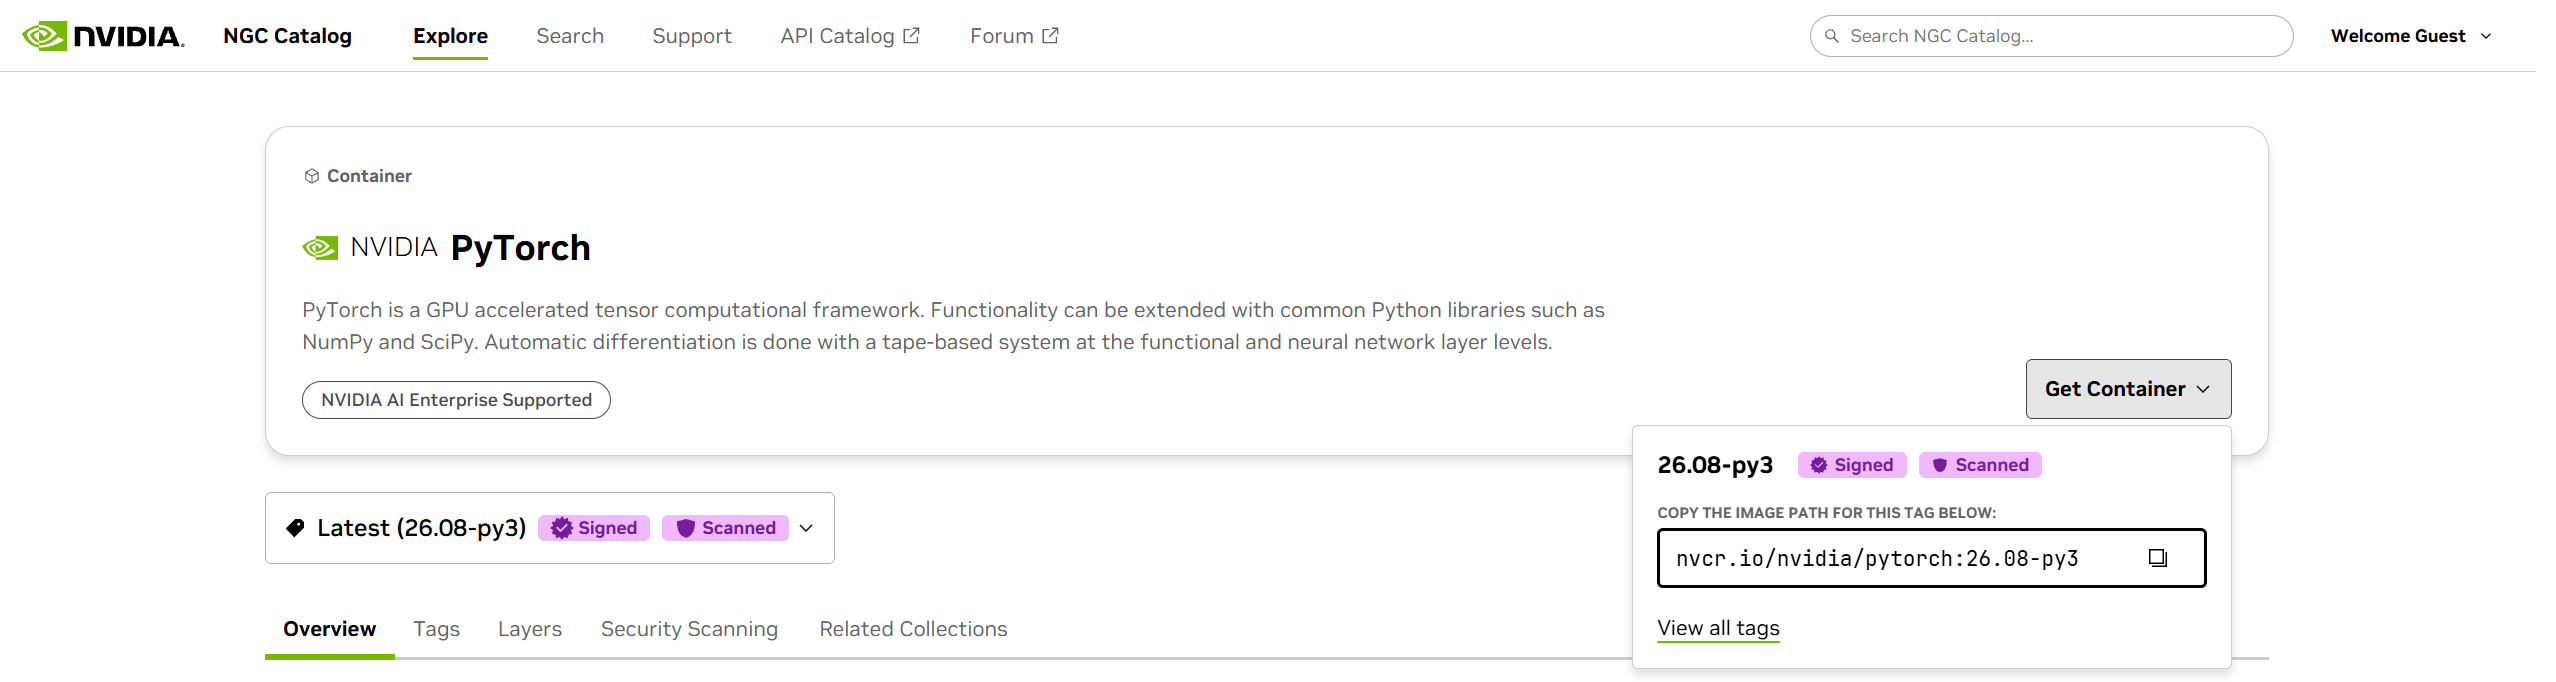
\includegraphics[width=\linewidth]{figures/container.png}
  \caption{Example container image source.}
  \label{fig:container-image-source}
\end{figure}

\section{Create a Python Environment in the Container}
\label{sec:setting-container}
The container image is normally read-only. The following workflow makes the project directory visible inside the container at \texttt{/workspace} and stores a writable Python virtual environment there. The environment remains available after the container command ends.

\subsection{Define Paths and Install Dependencies}
\label{subsec:container-environment-setup}
Replace the project, image, and environment placeholders before running any command. Keep the same definitions throughout one terminal session.

The \texttt{--nv} option exposes the host NVIDIA driver and allocated GPU to the container. Use it only within a GPU allocation when the program requires a GPU.
\begin{lstlisting}[style=terminal]
# Define paths and retain these variables for the session.
PROJECT=/data/project/naruemon/your_project
IMAGE=$PROJECT/containers/your_container.sif
ENV_TAG=your_environment
VENV=/workspace/.venv-$ENV_TAG

# Verify GPU access inside the container.
singularity exec --nv \
  --bind "$PROJECT:/workspace:rw" \
  "$IMAGE" \
  nvidia-smi

# Create the virtual environment.
singularity exec --nv \
  --bind "$PROJECT:/workspace:rw" \
  "$IMAGE" \
  python -m venv "$VENV"

# Install PyTorch from the selected CUDA wheel index.
singularity exec --nv \
  --bind "$PROJECT:/workspace:rw" \
  "$IMAGE" \
  "$VENV/bin/python" -m pip install --no-cache-dir \
  torch torchvision \
  --index-url https://download.pytorch.org/whl/cu126

# Install the remaining project dependencies.
singularity exec --nv \
  --bind "$PROJECT:/workspace:rw" \
  "$IMAGE" \
  "$VENV/bin/python" -m pip install --no-cache-dir \
  -r /workspace/requirements.txt

# Uninstall packages listed in the same requirements file.
singularity exec --nv \
  --bind "$PROJECT:/workspace:rw" \
  "$IMAGE" \
  "$VENV/bin/python" -m pip uninstall -y \
  -r /workspace/requirements.txt

# Completely reset the project-specific virtual environment.
rm -rf -- "$PROJECT/.venv-$ENV_TAG"
\end{lstlisting}

The \texttt{--bind} option maps the project directory to \texttt{/workspace} inside the container. The selected PyTorch package must support the allocated GPU and the host NVIDIA driver.

The final two groups of commands in the example are maintenance operations, not normal installation steps. The uninstall command removes packages, and the reset command permanently deletes the project-specific virtual environment. Run either operation only when you intentionally need to repair or recreate that environment, and verify the resolved project path first.

\section{Run a Container in a Batch Job}
\label{subsec:container-sbatch}

A containerized program uses the same Slurm resource directives as any other batch job. The job must request a GPU when \texttt{singularity exec --nv} is used. Replace the project-specific paths in the example before submission.
\begin{lstlisting}[language=bash]
#!/bin/bash -l
#SBATCH --job-name=mtj
#SBATCH --partition=gpu
#SBATCH --qos=gpu40g24m
#SBATCH --gres=gpu:7g.40gb:2
#SBATCH --mem=20G
#SBATCH --cpus-per-task=2
#SBATCH --output=mtj-%j.out
#SBATCH --error=mtj-%j.err
mkdir -p logs

set -euo pipefail

PROJECT=/data/project/naruemon/your_project
IMAGE=$PROJECT/containers/your_container.sif
ENV_TAG=your_environment
VENV=/workspace/.venv-$ENV_TAG


singularity exec --nv \
  --pwd /workspace \
  --bind "$PROJECT:/workspace:rw" \
  "$IMAGE" \
  "$VENV/bin/python" \
  /workspace/script1.py


\end{lstlisting}


\section{Run a Container Interactively}
\label{subsec:container-srun}

First request an interactive allocation with a permitted partition, QoS, and GPU profile:
\begin{lstlisting}[style = terminal]
  srun -p gpu -c2 --mem=8G --qos=gpu40g24m --gres=gpu:7g.40gb:1 --pty bash -l
\end{lstlisting}
After the allocation starts, define the project, image, and environment paths:
\begin{lstlisting}[style = terminal]
PROJECT=/data/project/naruemon/your_project
IMAGE=$PROJECT/containers/your_container.sif
ENV_TAG=your_environment
VENV=/workspace/.venv-$ENV_TAG
\end{lstlisting}
Run the program inside the container. Retain \texttt{--nv} for GPU work; omit it for CPU-only work:
\begin{lstlisting}[style = terminal]
  singularity exec --nv \
  --pwd /workspace \
  --bind "$PROJECT:/workspace:rw" \
  "$IMAGE" \
  "$VENV/bin/python" \
  /workspace/script1.py
\end{lstlisting}

\vfill
\begin{center}

\textit{“When life leaves us blind, love keeps us kind.”}

--- Chester Bennington
\end{center}



\backmatter


\end{document}
